\documentclass[11pt, oneside]{article}   	% use "amsart" instead of "article" for AMSLaTeX format
\usepackage{geometry}                		% See geometry.pdf to learn the layout options. There are lots.
\geometry{letterpaper}                   		% ... or a4paper or a5paper or ... 
%\geometry{landscape}                		% Activate for for rotated page geometry
%\usepackage[parfill]{parskip}    		% Activate to begin paragraphs with an empty line rather than an indent
\usepackage{graphicx}				% Use pdf, png, jpg, or eps� with pdflatex; use eps in DVI mode
\usepackage{amsmath}								% TeX will automatically convert eps --> pdf in pdflatex		
\usepackage{amssymb}
\setlength{\parindent}{0cm}

\title{Families of RV}
\author{Yulong Yang}
%\date{}							% Activate to display a given date or no date

\begin{document}
\maketitle
%\section{}
%\subsection{}

\section{Gaussian Random Variables}

Gaussian $(\mu, \sigma)$ random variable $X$ has mean $\mu$ and variance $\sigma^2$ ($\sigma > 0$), and has PDF, 

\begin{equation}
f_X(x) = \frac{1}{\sqrt{2\pi\sigma^2} }e^{-(x-\mu)^2/2\sigma^2 }
\end{equation}

Standard normal $(0,1)$ RV is when Gaussian RV has $\mu=0, \sigma=1$, and its CDF is,

\begin{equation}
\Phi (x) = \frac{1}{\sqrt{2\pi} }\int_{-\infty}^x e^{-u^2/2du}
\end{equation}

Therefore, for general $F_X(x)$, by replacing $z = \frac{x-\mu}{\sigma}$, we have,

\begin{equation}
F_X(x) = P[X \leq x] = \Phi (\frac{x-\mu}{\sigma})
\end{equation}

and,

\begin{equation}
\Phi (-x) = P[X > x] = 1 - \Phi (x)
\end{equation}

\begin{equation}
P[a < X \leq b] = \Phi (\frac{b-\mu}{\sigma}) - \Phi (\frac{a-\mu}{\sigma})
\end{equation}

also, if $X$ is Gaussian $(\mu, \sigma)$ random variable, then $Y = aX + b$ is Gaussian $(a\mu+b, a\sigma)$ RV.


Gaussian RV is,

\begin{itemize}
\item additive
\item continuous
\end{itemize}

\section{Detection error}

When we try to detect a signal, it is either present ($s_1$) or absent ($s_0$). When present the mean could be $A$, and $0$ when absent, as the Figure~\ref{fig:detection}. 

\begin{figure}[htpb]
\begin{center}
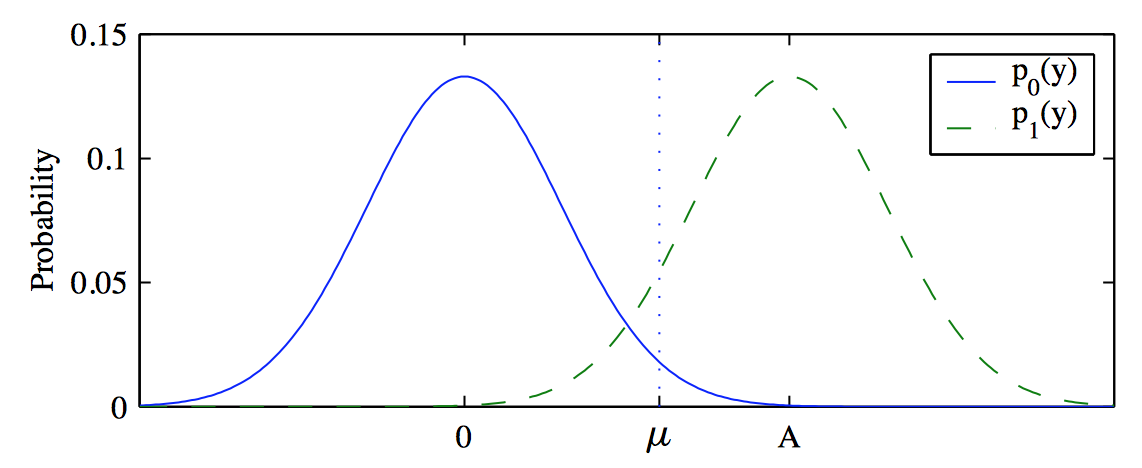
\includegraphics[width=\textwidth]{detection.png}
\caption{Master Therorem}
\label{fig:detection}
\end{center}
\end{figure}

In such detection scenario, we have two types of detection error,

\begin{itemize}
\item false alarm: $P(detecting\_as\_s_1 | s_0)$
\item missed detection: $P(detecting\_as\_s_0 | s_1)$
\end{itemize}

Therefore, let $P_1, P_0$ be the probability of the signal present and absent respectively, the probability of detection error is,

\begin{equation}
P_e = P_0P(detecting\_as\_s_1 | s_0) + P_1P(detecting\_as\_s_0 | s_1)
\end{equation}

\section{Point estimate}

Let $X$ be a Gaussian $(\mu, \sigma)$ RV. A confidence interval estimate would be

\begin{equation}
M_n(X) - c \leq \mu \leq M_n(X) + c
\end{equation}

in which $M_n(X)$ is the estimate of $\mu$, and $n$ is the sample size. It is equivalent to 

\begin{equation}
|\mu - M_n(X)| \leq c
\end{equation}

To convert it into z-score,

\begin{equation}
z = \frac{M_n(X) - \mu}{\sigma / \sqrt{n}}
\end{equation}

The estimate has a confidence coefficient $1-\alpha$ where

\begin{equation}
\alpha/2 = 1 - \Phi (\frac{c\sqrt{n}}{\sigma})
\end{equation}

and once we get $c$ from $\Phi()$, we could calculate either $M_n$ or $n$.


\end{document}  